\chapter{Atmospheric Data Fitting}
\label{app:appendixB-fittingProcessAndResults}
In \Cref{subsec:atmofuncfit} the final results of the atmospheric data fits were presented. However, before those results could be obtained, a few iterations of trial-and-error fits were required. These intermediate trials are presented for both the temperature data, in \Cref{appsec:tempFit}, as well as for the density data, in \Cref{appsec:denFit}. The fit requirements for the polynomial function were set such that the errors created by the fit were less than the uncertainty of the latitude and longitude dependent data. This way the desired accuracy could still be reached. This uncertainty is caused by the difference in atmospheric data curves for the different latitudes and longitudes. The atmospheric data curve for the latitude and longitude corresponding to the launch site (21.0 $^\circ$N and 74.5 $^\circ$E) was taken as the reference curve and called the launch site curve. The differences between this launch site curve and the 8 other curves were used to define the maximum data curves difference. The \textit{polyfit.m} function within Matlab was used to fit a polynomial to the data. This function also directly provides a standard deviation of the fit for each data point (in combination with the \textit{polyval.m} function). One of the requirement was for the maximum standard deviation of the polynomial fit to be one order less than the maximum difference of the data curves with respect to the launch site curve. The second requirements for a proper fit was for the absolute maximum difference between the polynomial fit and the launch site curve to be less than the absolute maximum difference between the data curves and that same launch site curve. 


\section{Temperature}
\label{appsec:tempFit}
Initially, the temperature data curve was split into 6 different sections as portrayed in \Cref{fig:temperatureDataSplit6}. The sections were selected on the basis of their individual shapes and the maximum order that was required, where the maximum order for temperature was set at 8. Fewer sections were however always preferred. 

\begin{figure}[!ht]
\centering
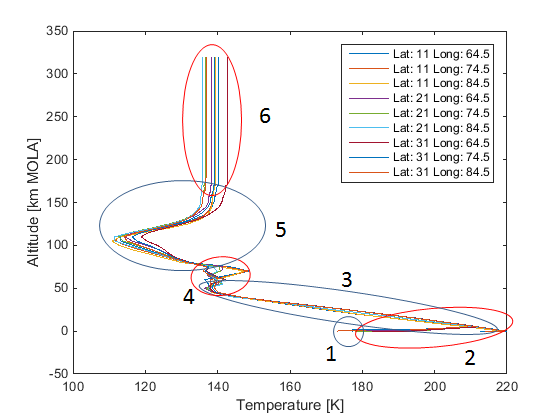
\includegraphics[width=0.8 \textwidth]{figures/software/temperatureDataSplit6.png}
\caption{Six different temperature curve sections}
\label{fig:temperatureDataSplit6}
\end{figure}

\noindent
Unfortunately, the fourth quarter of section 3 caused this section to not meet the maximum standard deviation requirement because in that quarter the linear behaviour changes directions slightly and the differences between the different data curves become a lot smaller. Therefore section 3 was split into two different sections resulting in a total of 7 sections as shown in \Cref{fig:temperatureDataSplit7}.

\begin{figure}[H]
\centering
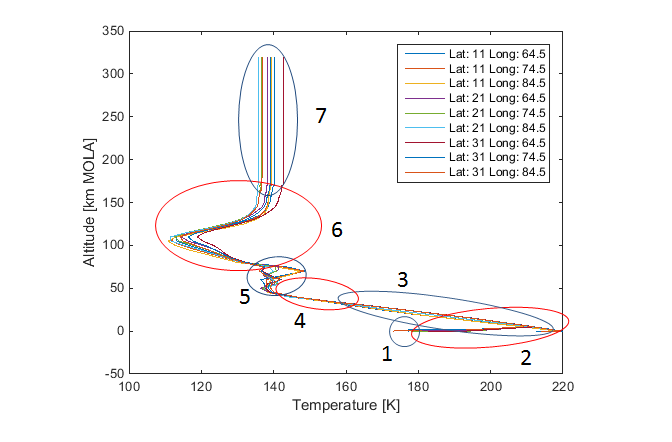
\includegraphics[width=1.0 \textwidth]{figures/software/temperatureDataSplit7.png}
\caption{Seven different temperature curve sections}
\label{fig:temperatureDataSplit7}
\end{figure}



\begin{figure}[H]
\centering
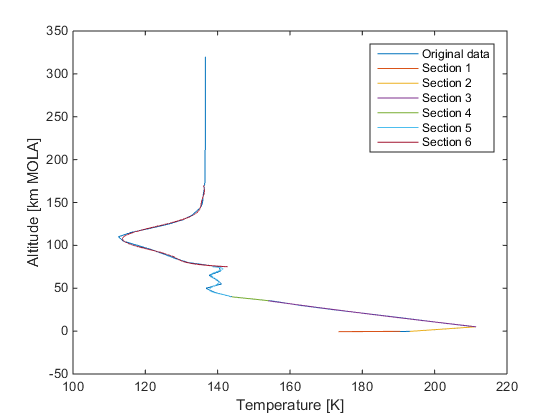
\includegraphics[width=0.6 \textwidth]{figures/software/completePolyFitTempSplit7.png}
\caption{All section fits for the launch site temperature data curve}
\label{fig:completePolyFitTempSplit7}
\end{figure}

\noindent
These sections all met the requirements and thus provided a proper fit to the data. This fit is shown in \Cref{fig:completePolyFitTempSplit7}.


However, because fewer sections were preferred, an attempt was made to reduce the number of sections. Because of the inaccuracy in the Mars-\ac{GRAM} model close to the planet surface, it was decided to delete the outliers near the surface (section 1) and stretch the outcome of the second polynomial fit to the surface instead. Also, it turned out that section 4 and 5 could be combined in such a way that the requirements were still met. This reduced the number of sections from 7 to 5. The final fit was presented in \Cref{subsec:atmofuncfit} as well as the corresponding errors and polynomial coefficients.                                                                                      




\section{Density}
\label{appsec:denFit}
For the density curve, because the data represents a logarithmic curve, initially an exponential atmosphere was fit. However, this did not meet any of the requirements for a proper fit. This is why a polynomial fit was attempted for the density curve as well with the same requirement as the temperature fits. The first fit was attempted with two sections as presented in \Cref{fig:densityDataSplit2}. 

\begin{figure}[H]
\centering
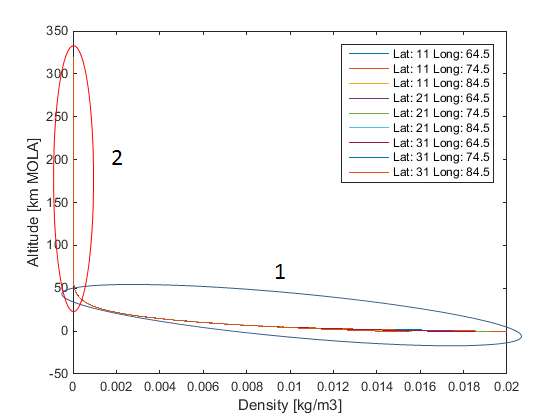
\includegraphics[width=0.69 \textwidth]{figures/software/densityDataSplit2.png}
\caption{Two different density curve sections}
\label{fig:densityDataSplit2}
\end{figure}



\begin{figure}[H]
\centering
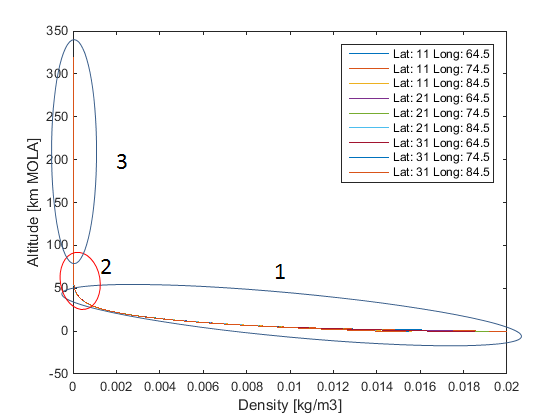
\includegraphics[width=0.7 \textwidth]{figures/software/densityDataSplit3.png}
\caption{Three different density curve sections}
\label{fig:densityDataSplit3}
\end{figure}

\noindent
However, the second section could not meet the requirements because of the initial part. This is why it was split into three sections as presented in \Cref{fig:densityDataSplit3}. This did meet the error requirements and resulted in the fit as shown in \Cref{fig:completePolyFitDenSplit3} with section 1 being the lower part, section 2 the middle and section 3 the upper part. However, in this case the fit for section three resulted in an oscillating behaviour around the actual data which caused the density values to drop below zero as shown in \Cref{fig:section3PolyFitDen}. Since this is unrealistic, an exponential atmospheric fit for only the third section was attempted (also shown in \Cref{fig:section3PolyFitDen}) however, this resulted in the same behaviour as the attempt for the entire curve. Therefore, it was decided to try a different exponential approach which eventually resulted in the fit described in \Cref{subsec:atmofuncfit}.

\Cref{fig:ExpAtmFitDenZoom} clearly shows that both the full exponential atmospheric fit and the polynomial fits were not a proper choice here. The figure shows the curved part of the curve.

\begin{figure}[H]
\centering
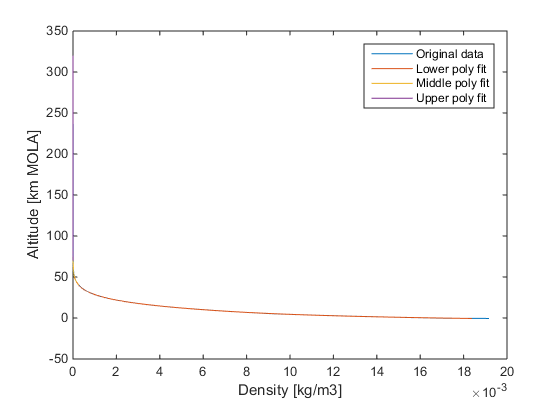
\includegraphics[width=0.7 \textwidth]{figures/software/completePolyFitDenSplit3.png}
\caption{All section fits for the launch site density data curve}
\label{fig:completePolyFitDenSplit3}
\end{figure}

 

\begin{figure}[H]
\centering
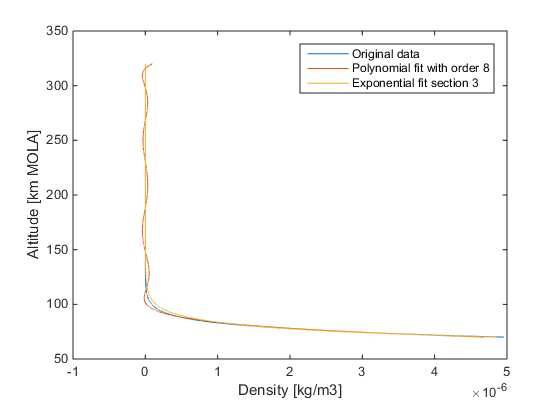
\includegraphics[width=0.7 \textwidth]{figures/software/section3PolyFitDen.png}
\caption{Section 3 fit for the launch site density data curve}
\label{fig:section3PolyFitDen}
\end{figure}



\begin{figure}[H]
\centering
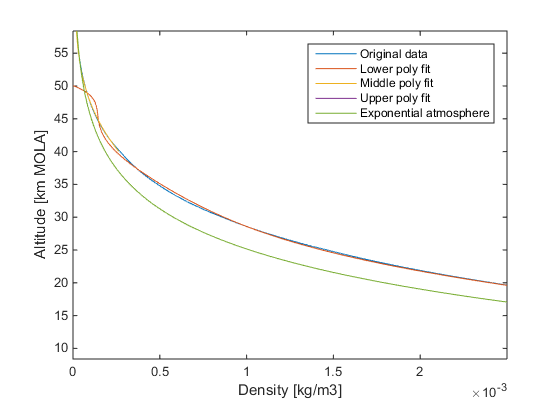
\includegraphics[width=0.7 \textwidth]{figures/software/ExpAtmFitDenZoom.png}
\caption{Zoom in of the end of section 1 with the polynomial and exponential atmospheric fits}
\label{fig:ExpAtmFitDenZoom}
\end{figure}

